%--------------------------------------------------------------------%
% Bab II — Studi Literatur
% @author Refki Alfarizi
%--------------------------------------------------------------------%

\chapter{Studi Literatur}
\label{chap:studi-literatur}

Bab ini berisi studi literatur yang berkaitan dengan topik persoalan tugas akhir untuk memberikan informasi mengenai dasar teori dan studi yang digunakan. Bab ini diharapkan dapat membantu pembaca untuk lebih memahami penelitian tugas akhir ini.

\section{Kompatibilitas Perangkat Lunak}
\label{sec:kompatibilitas}

Pustaka perangkat lunak adalah kumpulan kode yang menyediakan fungsi untuk digunakan kembali oleh program lain\@. \textit{Application programming interface} (API) adalah antarmuka yang menetapkan operasi pustaka yang disediakan untuk program pengguna beserta cara menggunakannya. Program pengguna tersebut disebut klien. Selama pengembangan, pustaka mengalami perubahan untuk menambah fungsi, memperbaiki kesalahan, atau menyesuaikan kebutuhan penggunanya. Perubahan ini dapat memengaruhi klien ketika versi pustaka yang digunakan diperbarui \parencite{Ochoa2023}.

\textit{Backward compatibility} adalah kemampuan versi baru pustaka untuk menggantikan versi lama tanpa mengganggu penggunaan yang sebelumnya didukung. Kompatibilitas ini berkaitan dengan deklarasi API dan kontrak perilakunya. Kontrak perilaku menjelaskan masukan yang diterima, hasil yang dijamin, serta perubahan keadaan program setelah API dipanggil. Berdasarkan prinsip substitusi perilaku, penggantian yang kompatibel tidak memperketat prasyarat pemanggilan atau memperlemah jaminan hasil bagi penggunaan yang sudah didukung \parencite{LiskovWing1994,Ochoa2023}.

\subsection{Jenis Kompatibilitas dan \textit{Breaking Changes}}

\textit{Breaking change} (BC) adalah perubahan yang menyebabkan penggunaan pustaka yang sebelumnya didukung menjadi tidak kompatibel. Dampaknya pada klien bergantung pada API yang digunakan dan kondisi pemanggilannya. Dalam bahasa pemrograman Java, kompatibilitas dapat dibedakan menjadi tiga jenis berikut \parencite{Ochoa2023,JLS25Chapter13}.

\begin{enumerate}
    \item \textit{Source compatibility}, yaitu kemampuan kode sumber klien lama untuk tetap dikompilasi terhadap versi baru pustaka.
    \item \textit{Binary compatibility}, yaitu kemampuan biner klien yang telah dikompilasi untuk tetap ditautkan tanpa kesalahan setelah pustaka diganti.
    \item \textit{Behavioral compatibility}, yaitu kemampuan versi baru untuk mempertahankan kontrak perilaku API bagi penggunaan yang sebelumnya didukung.
\end{enumerate}

Dua jenis pertama berkaitan dengan struktur API\@. Perubahan yang merusak \textit{source compatibility} atau \textit{binary compatibility} disebut BC sintaktis \parencite{Ochoa2023}. Penghapusan metode dapat menyebabkan kode sumber klien gagal dikompilasi atau biner klien gagal ditautkan. Sebaliknya, perubahan perhitungan di dalam metode dapat menghasilkan nilai berbeda tanpa mengubah deklarasi metode. Oleh karena itu, keberhasilan kompilasi dan penautan belum menjamin bahwa kontrak perilaku API tetap terpenuhi \parencite{JLS25Chapter13}.

\textit{Semantic Versioning} (SemVer) adalah skema penomoran versi untuk mengomunikasikan jenis perubahan dan kompatibilitas suatu rilis. Nomor versinya terdiri atas komponen mayor, minor, dan \textit{patch}. Untuk API stabil, perubahan yang tidak kompatibel ditandai dengan kenaikan versi mayor, penambahan fungsi yang kompatibel dengan kenaikan versi minor, dan perbaikan kesalahan yang kompatibel dengan kenaikan versi \textit{patch}. Versi mayor nol digunakan untuk tahap pengembangan awal \parencite{SemVer200}. Penomoran tersebut menyampaikan jaminan pengembang, tetapi tidak memverifikasi kompatibilitas implementasi secara otomatis.

\subsection{\textit{Behavioral Breaking Changes}}
\label{subsec:behavioral-bc}

\textit{Behavioral breaking change}, yang juga disebut BC semantik, adalah perubahan yang melanggar kontrak perilaku API\@. Perubahan ini dapat memengaruhi nilai kembalian, eksepsi yang dilempar, keadaan objek, atau efek samping seperti penulisan berkas. API publik adalah antarmuka yang disediakan pustaka untuk klien, sedangkan metode internal adalah metode pendukung di luar antarmuka tersebut. Penyebab BC dapat berada di dalam metode API publik maupun metode internal yang dipanggilnya. Karena deklarasi API dapat tetap sama, pemeriksaan struktur API saja tidak cukup untuk menemukan perubahan semacam ini \parencite{Ochoa2023}.

Sebagai ilustrasi, kontrak suatu API registrasi menetapkan bahwa pengguna dengan usia minimal 18 tahun dapat diterima. Jika kondisi validasi berubah dari \texttt{age >= 18} menjadi \texttt{age >= 21}, pengguna berusia 18--20 tahun yang sebelumnya diterima akan ditolak. Perubahan ini melanggar kontrak tersebut meskipun deklarasi metodenya tetap sama.

Perbedaan hasil tidak selalu menandakan BC\@. Jika kontrak sejak awal menetapkan batas 21 tahun, perubahan pada contoh tadi dapat merupakan koreksi terhadap implementasi yang keliru. Demikian pula, penambahan fungsi dapat mengubah hasil untuk masukan yang sebelumnya tidak didukung tanpa mengganggu penggunaan lama. Penilaian kompatibilitas karena itu didasarkan pada kontrak yang hendak dipertahankan, bukan pada tuntutan agar seluruh hasil kedua versi selalu sama \parencite{Ochoa2023}.

\section{Analisis Statis dan Dampak Perubahan}
\label{sec:analisis-statis}

Analisis statis adalah teknik pemeriksaan sifat program tanpa mengeksekusi program tersebut. Analisis ini menggunakan model kode untuk menelaah kemungkinan perilaku program saat dijalankan \parencite{Nielson1999}. Pada program Java, analisis dapat dilakukan terhadap kode sumber atau \textit{bytecode}, yaitu kode antara hasil kompilasi untuk mesin virtual Java \parencite{JLS25Chapter13}.

\subsection{Representasi Program untuk Analisis Perubahan}

Representasi program adalah model yang menggambarkan unsur kode, seperti metode atau pernyataan, beserta hubungan di antaranya. Dalam analisis perubahan, model ini digunakan untuk membandingkan struktur kode antarversi serta menelusuri keterkaitan bagian yang berubah dengan bagian lain.

\textit{Abstract syntax tree} (AST) adalah struktur pohon yang merepresentasikan susunan sintaksis kode sumber. Setiap unsur pada pohon, yang disebut simpul, mewakili konstruksi program, seperti deklarasi, ekspresi, dan percabangan. Garis penghubung antarsimpul, yang disebut sisi, menunjukkan hubungan hierarkis antarkonstruksi tersebut. Perbandingan AST dapat menghasilkan rangkaian operasi penyuntingan pada struktur kode, antara lain penyisipan, penghapusan, pembaruan, dan pemindahan simpul \parencite{Falleri2014}. Gambar~\ref{fig:ast-comparison} memperlihatkan contoh kode Java dan AST pada dua versi. Garis putus-putus yang menghubungkan kedua AST menandai pasangan simpul yang bersesuaian.

\begin{figure}[htbp]
    \centering
    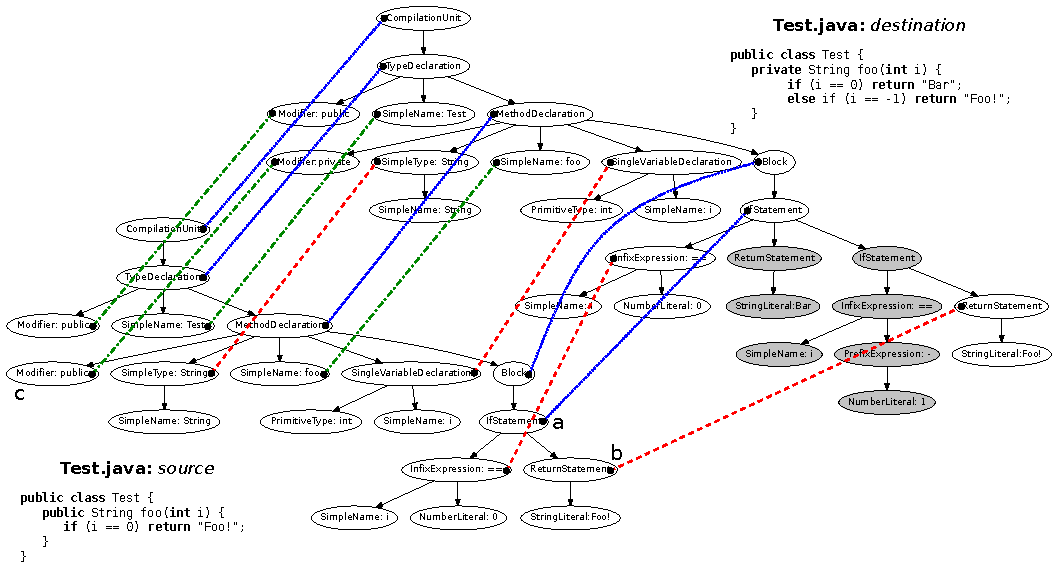
\includegraphics[width=\textwidth]{resources/figures/ast-comparison-original.pdf}
    \caption[Contoh kode Java dan representasi AST]{Contoh kode Java dan representasi AST pada dua versi \parencite{Falleri2014}.}
    \label{fig:ast-comparison}
\end{figure}

Perbandingan AST menunjukkan perubahan struktur kode, tetapi belum menjelaskan pengaruhnya terhadap perilaku program. Untuk menelusuri hubungan antarmetode, digunakan \textit{call graph}, yaitu graf berarah yang merepresentasikan kemungkinan pemanggilan. Dalam bentuk sederhananya, simpul mewakili metode, sedangkan sisi dari metode A menuju metode B menunjukkan bahwa A dapat memanggil B. Penelusuran dari API publik dapat menemukan metode yang dipanggil secara langsung maupun tidak langsung. Penelusuran dalam arah sebaliknya dapat menemukan API publik yang memanggil suatu metode internal \parencite{GroveChambers2001}.

Di dalam metode, kemungkinan alur eksekusi direpresentasikan oleh \textit{control-flow graph} (CFG). Simpul pada graf berarah ini mewakili pernyataan atau kelompok pernyataan, sedangkan sisinya menunjukkan kemungkinan perpindahan alur di antara simpul tersebut. Representasi ini memperlihatkan jalur eksekusi yang terbentuk oleh percabangan maupun perulangan \parencite{Tip1995}.

Untuk menelaah pengaruh suatu operasi terhadap operasi lain, digunakan \textit{program dependence graph} (PDG), yaitu graf yang merepresentasikan operasi program beserta ketergantungan data dan kendalinya. Ketergantungan data menyatakan hubungan antara operasi penghasil nilai dan operasi yang menggunakan nilai tersebut. Ketergantungan kendali menunjukkan bahwa pelaksanaan suatu operasi bergantung pada hasil percabangan \parencite{Ferrante1987}. Pada validasi usia, nilai parameter digunakan dalam operasi pembandingan, lalu hasil pembandingan menentukan apakah registrasi diterima atau ditolak.

Hubungan ketergantungan dapat digunakan untuk memilih bagian kode yang relevan melalui \textit{program slicing}. Teknik analisis ini memilih bagian program yang berkaitan dengan satu atau beberapa variabel pada titik program tertentu. Variabel dan titik tersebut menjadi kriteria pemilihan\@. \textit{Backward slicing} mencari pernyataan yang dapat memengaruhi nilai variabel pada titik itu, sedangkan \textit{forward slicing} mencari pernyataan yang nilai atau pelaksanaannya dapat dipengaruhi oleh kriteria tersebut. Jika penelusuran melintasi pemanggilan metode, hubungan parameter, nilai kembalian, dan data yang digunakan bersama juga diperhitungkan \parencite{Tip1995}.

\subsection{\textit{Change Impact Analysis}}

\textit{Change impact analysis} (CIA) adalah analisis untuk mengidentifikasi bagian perangkat lunak yang mungkin dipengaruhi oleh suatu perubahan. Analisis dimulai dari bagian yang berubah, kemudian menelusuri hubungan pemanggilan atau ketergantungan untuk menemukan bagian yang berpotensi terdampak. Hasilnya dapat digunakan untuk membantu pengujian dan peninjauan perubahan \parencite{RyderTip2001}.

Pada pustaka, perubahan metode internal dapat memengaruhi API publik yang memanggilnya. Namun, hubungan pemanggilan belum menunjukkan bahwa hasil API pasti berubah. Bagian yang disunting harus dapat dijalankan pada setidaknya salah satu versi, dan pengaruhnya harus mencapai nilai kembalian, eksepsi, atau keadaan yang dapat diamati pemanggil. Sebagai contoh, perubahan batas usia dalam metode bantu tidak memengaruhi hasil jika API pemanggil hanya meneruskan masukan berusia minimal 21 tahun pada kedua versi.

Ketepatan hasil CIA bergantung pada hubungan program yang berhasil dimodelkan. Pendekatan konservatif dapat memasukkan kemungkinan pemanggilan yang tidak terjadi saat program dijalankan \parencite{GroveChambers2001}. Sebaliknya, hubungan yang tidak teridentifikasi dapat menyebabkan dampak terlewat. Oleh karena itu, daftar bagian yang berpotensi terdampak masih perlu dianalisis untuk menentukan apakah perubahan perilakunya melanggar kontrak API\@.

\section{\textit{Large Language Model} untuk Analisis Kode}
\label{sec:llm}

\textit{Large language model} (LLM) adalah model bahasa yang dilatih pada data berskala besar untuk mempelajari pola urutan token. Token merupakan satuan teks yang diproses model dan dapat berupa kata, bagian kata, atau karakter. Berdasarkan konteks masukan, model menghasilkan urutan token sebagai respons. Pelatihan pada kode program memungkinkan model mempelajari pola kode dan hubungannya dengan deskripsi bahasa alami \parencite{Chen2021Code}.

\textit{Prompt} adalah masukan yang diberikan kepada LLM untuk mengarahkan responsnya. Isinya dapat berupa instruksi, kode, dan informasi pendukung. Salah satu bentuk informasi perubahan adalah \textit{diff}, yaitu representasi perbedaan kode antara dua versi. Dalam analisis perubahan, model dapat menerima implementasi kedua versi, \textit{diff}, dan kode metode yang berkaitan untuk diminta menjelaskan perubahan hasil atau kondisi pemicunya. Ketepatan penjelasan bergantung pada kemampuan model dan informasi yang tersedia; kode metode lain atau kontrak yang tidak diberikan dapat membatasi penilaian.

Model memiliki batas panjang masukan, dan kemampuannya memanfaatkan informasi juga dapat dipengaruhi oleh posisi informasi di dalam konteks \parencite{Liu2024LostMiddle}. Pemilihan bagian kode yang relevan membantu memusatkan konteks pada persoalan yang dianalisis. Dalam analisis kompatibilitas, penjelasan model perlu diperiksa terhadap kode dan kontrak API agar asumsi yang dihasilkan model tidak dianggap sebagai perilaku yang dijamin pustaka.

\section{Evaluasi Deteksi \textit{Breaking Changes}}
\label{sec:evaluasi-bc}

Klasifikasi biner adalah proses menetapkan suatu contoh ke salah satu dari dua kelas. Dalam deteksi BC, kelas positif menyatakan adanya BC, sedangkan kelas negatif menyatakan tidak adanya BC menurut jenis kompatibilitas yang diperiksa. Label acuan adalah kelas yang telah ditetapkan berdasarkan kriteria pelabelan dan digunakan untuk menilai prediksi. Pada analisis tingkat API, satu contoh dapat berupa pasangan API dari versi lama dan versi baru.

Hasil klasifikasi terdiri atas \textit{true positive} (TP), yaitu kasus positif yang dikenali dengan benar; \textit{false positive} (FP), yaitu kasus negatif yang salah dinyatakan positif; \textit{false negative} (FN), yaitu kasus positif yang terlewat; dan \textit{true negative} (TN), yaitu kasus negatif yang dikenali dengan benar.

\begin{samepage}
\textit{Precision} adalah proporsi peringatan BC yang benar, sedangkan \textit{recall} adalah proporsi BC yang berhasil ditemukan. F1 merupakan rata-rata harmonik keduanya. Ketiga ukuran tersebut dihitung menggunakan Persamaan~\ref{eq:metrik-bc} \parencite{Manning2008}.
\begin{equation}
    P = \frac{TP}{TP+FP}, \qquad
    R = \frac{TP}{TP+FN}, \qquad
    F_1 = \frac{2PR}{P+R}.
    \label{eq:metrik-bc}
\end{equation}

\end{samepage}

Rumus tersebut berlaku jika penyebutnya tidak nol. Kasus positif dan negatif diperlukan untuk menilai kemampuan menemukan BC sekaligus menghindari peringatan yang salah.

\section{Studi Terkait}
\label{sec:studi-terkait}

Berikut adalah beberapa penelitian yang telah dilakukan sebelumnya dan berkaitan dengan persoalan tugas akhir ini.

\subsection{\textit{Break the Code? Breaking Changes and Their Impact on Software Evolution}}
\label{subsec:ochoa}

\textcite{Ochoa2023} mengkaji evolusi pustaka dan dampak \textit{breaking changes} terhadap klien. Penelitian ini menghasilkan Maracas, alat analisis statis yang menerima dua versi pustaka Java dalam bentuk \textit{Java Archive} (JAR), yaitu arsip distribusi program Java, beserta kode sumber klien. Maracas membandingkan deklarasi API menggunakan alat japicmp, kemudian memeriksa penggunaan API dalam AST klien yang dibangun dengan Spoon, sebuah pustaka analisis kode Java. Hasilnya menunjukkan lokasi kode klien yang dapat menjadi tidak valid akibat perubahan API\@.

Pada kumpulan kasus \textit{comp-changes}, Maracas memperoleh \textit{precision} 0,96 dan \textit{recall} 0,95 dalam mengidentifikasi penggunaan API yang tidak valid. Salah satu batasannya berkaitan dengan refleksi, yaitu mekanisme untuk memeriksa atau mengakses kelas dan anggotanya saat program berjalan. Maracas belum menganalisis penggunaan mekanisme ini dan dapat terkendala oleh informasi hierarki pewarisan yang tidak lengkap \parencite[hlm.~192--194]{Ochoa2023}. Kemampuan Maracas juga digunakan oleh BreakBot untuk melaporkan dampak perubahan saat pengembang meninjau usulan perubahan pustaka \parencite{Ochoa2022BreakBot}.

Analisis Maracas berfokus pada BC sintaktis dan lokasi penggunaannya dalam kode klien. Perubahan perilaku yang tidak mengubah struktur API belum menjadi sasaran analisis tersebut. Disertasi tersebut menempatkan deteksi BC semantik dan penelusuran dampaknya pada klien sebagai arah penelitian lanjutan \parencite[hlm.~208]{Ochoa2023}.

\subsection{\textit{Roseau: Fast, Accurate, Source-based API Breaking Change Analysis in Java}}
\label{subsec:roseau}

\textcite{Latappy2025Roseau} mengembangkan Roseau untuk memeriksa \textit{source compatibility} dan \textit{binary compatibility} API Java. Roseau mengekstraksi model API dari kode sumber atau \textit{bytecode}, lalu membandingkan model kedua versi. Pada 267 kasus sintetis, alat ini memperoleh F1 keseluruhan 0,99 untuk membedakan perubahan yang bersifat \textit{breaking} dari perubahan yang kompatibel.

Berbeda dari Maracas yang juga menelusuri penggunaan API pada klien, Roseau berfokus pada perbandingan API pustaka. Isi metode tidak diperiksa sehingga perubahan perilaku dengan deklarasi yang tetap kompatibel berada di luar cakupannya \parencite{Latappy2025Roseau}.

\subsection{\textit{Has My Release Disobeyed Semantic Versioning? Static Detection Based on Semantic Differencing}}
\label{subsec:sembid}

\textcite{Zhang2022Sembid} mengembangkan Sembid untuk mendeteksi BC semantik pada API Java antarversi. Alur analisisnya diringkas pada Gambar~\ref{fig:sembid-overview}. Sembid menelusuri rantai pemanggilan dari API publik menuju metode internal, kemudian menyusun ringkasan ketergantungan data, kendali, dan eksepsi. Ringkasan tersebut membentuk graf semantik yang menghubungkan pernyataan-pernyataan terkait melalui alur eksekusinya. Graf kedua versi lalu dibandingkan. Perbedaan yang sesuai dengan pola perubahan kompatibel diberi bobot lebih rendah untuk mengurangi peringatan yang salah.

\begin{figure}[htbp]
    \centering
    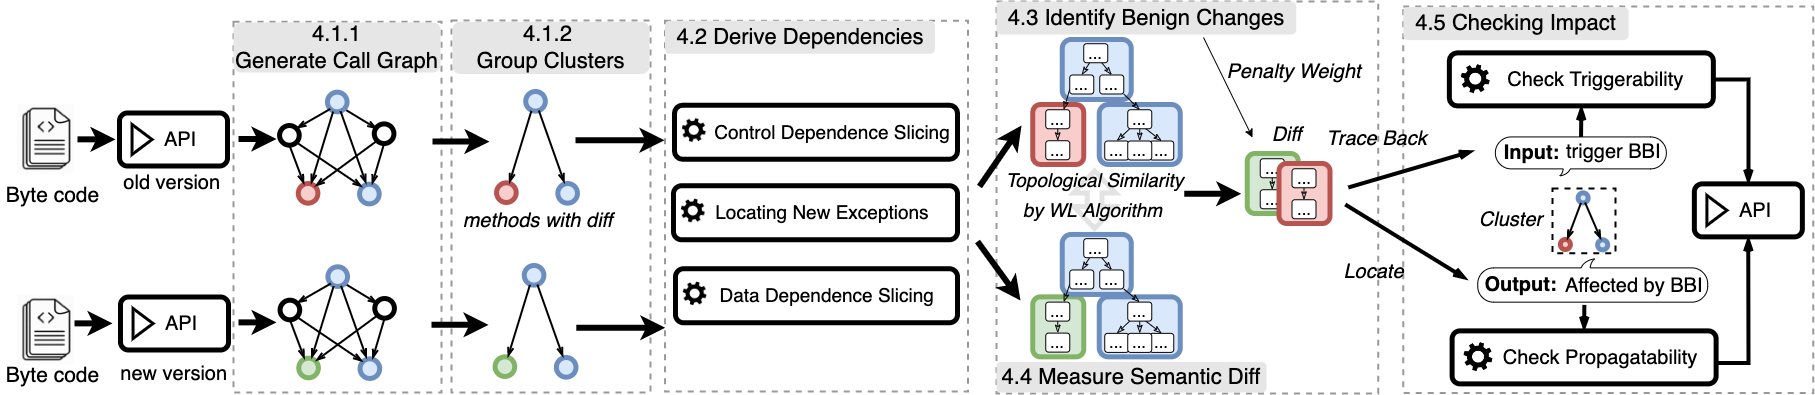
\includegraphics[width=\textwidth]{resources/figures/sembid-overview-original.png}
    \caption[Alur analisis Sembid]{Alur analisis Sembid \parencite{Zhang2022Sembid}.}
    \label{fig:sembid-overview}
\end{figure}

\begin{samepage}
Setelah menemukan perbedaan semantik, Sembid memeriksa \textit{triggerability} dan \textit{propagatability}. Pemeriksaan pertama menilai apakah perubahan dapat dipicu oleh masukan yang sebelumnya didukung. Pemeriksaan kedua menelusuri apakah pengaruhnya dapat mencapai keluaran API\@. Dengan demikian, analisisnya mencakup perubahan di dalam metode yang dipanggil API, bukan hanya perubahan pada metode publik itu sendiri.

\end{samepage}

Evaluasinya menggunakan 671 pasangan API dari 77 pasangan versi, terdiri atas 308 kasus positif dan 363 kasus negatif. Kasus positif mengandung BC semantik, sedangkan kasus negatif tidak mengandung BC semantik menurut kriteria studi tersebut, meskipun sebagian memiliki perubahan biner. Sembid memperoleh \textit{precision} 81,29\%, \textit{recall} 90,26\%, dan F1 85,54\%. Analisis kesalahan melaporkan 64 FP, termasuk 24 kasus implementasi ulang yang ekuivalen. Sebanyak 30 kasus positif terlewat; penyebabnya antara lain perubahan pencatatan log atau penulisan berkas, kesalahan pengenalan pola perubahan kompatibel, dan refleksi \parencite{Zhang2022Sembid}.

Berbeda dari pemeriksaan deklarasi pada Maracas dan Roseau, Sembid menganalisis hubungan perubahan implementasi dengan keluaran API tanpa memerlukan kode klien sebagai masukan utama. Kesalahan pada implementasi ulang yang ekuivalen menunjukkan batas pendekatannya: struktur komputasi dapat berbeda meskipun kontrak perilaku tetap terpenuhi.

\subsection{\textit{BCaLLM:\ Call Graph-Guided Python Breaking Change Detection with Large Language Models}}
\label{subsec:bcallm}

\textcite{Cheng2026BCaLLM} memperkenalkan BCaLLM yang menggabungkan \textit{call graph} dan LLM untuk mendeteksi BC pada paket Python. Implementasi resminya menggunakan hubungan pemanggilan pada dua versi untuk memilih konteks API yang dianalisis. Model menerima definisi API pada versi lama dan baru beserta konteks fungsi atau metode yang dipanggil. Hasil penilaian yang telah diperoleh disimpan sebagai ringkasan dan digunakan saat menganalisis API lain yang berkaitan \parencite{BCaLLMArtifact2026}.

BCaLLM menyediakan PyBCEval, yaitu dataset pembaruan paket Python untuk evaluasi deteksi BC, serta beberapa varian eksperimen, termasuk varian tanpa ringkasan. Ringkasan yang digunakan merupakan hasil penilaian LLM terhadap kompatibilitas API\@. Jenis informasi ini berbeda dari ringkasan ketergantungan yang dihitung secara statis oleh Sembid \parencite{BCaLLMArtifact2026}.

Sembid menilai perbedaan semantik dengan analisis program, sedangkan BCaLLM menggunakan struktur pemanggilan untuk mendukung penilaian LLM\@. Kedua pendekatan memperhitungkan kode internal yang dipanggil API\@. Namun, penerapannya pada bahasa dan kumpulan data yang berbeda membatasi perbandingan langsung atas hasil deteksinya.

\subsection{\textit{An Approach and Benchmark to Detect Behavioral Changes of Commits in Continuous Integration}}
\label{subsec:dci}

\textcite{Danglot2020DCI} mengembangkan DCI untuk menghasilkan tes yang membedakan perilaku program sebelum dan sesudah suatu \textit{commit}, yaitu rekaman perubahan dalam repositori kode. DCI memilih tes yang mengeksekusi kode yang berubah. Tes tersebut diperluas melalui \textit{assertion amplification}, yaitu penambahan pemeriksaan terhadap hasil atau keadaan program, serta eksplorasi variasi masukan. Pada 60 \textit{commit} dari enam proyek Java, konfigurasi amplifikasi berbasis pencarian menghasilkan tes pendeteksi perubahan untuk 25 \textit{commit}.

DCI bergantung pada keberadaan tes yang telah mengeksekusi bagian yang berubah sehingga tidak dapat diterapkan pada seluruh \textit{commit} \parencite{Danglot2020DCI}. Berbeda dari detektor BC, DCI mencari bukti perbedaan perilaku tanpa menentukan apakah perbedaan itu melanggar kompatibilitas. Tes yang membedakan dua versi dapat pula menunjukkan perubahan yang memang dikehendaki, seperti perbaikan kesalahan.

\subsection{\textit{BreakGuard: Towards Detecting Dependency Breaking Changes with LLM-Generated Tests}}
\label{subsec:breakguard}

\textcite{Raj2026BreakGuard} mengembangkan BreakGuard untuk mendeteksi kegagalan kompatibilitas saat pustaka diperbarui. BreakGuard menggunakan analisis statis untuk mengambil konteks metode klien yang memakai pustaka, lalu meminta LLM menghasilkan tes. Tes harus dapat dikompilasi dan lulus pada versi dependensi lama sebelum diperiksa pada versi baru. Evaluasinya menggunakan 89 kasus terpilih dari BUMP, sebuah dataset pembaruan dependensi Java. Konfigurasi GPT-4o dengan konteks kelas mendeteksi 27 kasus atau 30,3\%.

BreakGuard lebih berhasil mendeteksi galat saat eksekusi, seperti kelas atau metode yang tidak ditemukan, daripada perbedaan nilai yang membutuhkan pemeriksaan hasil tertentu. Kumpulan kasusnya berisi kegagalan pembaruan yang telah diketahui dan tidak seluruhnya berupa BC semantik. Karena itu, persentase deteksi tersebut tidak dapat disamakan dengan F1 pada klasifikasi kasus positif dan negatif \parencite{Raj2026BreakGuard}.

Seperti DCI, BreakGuard menggunakan eksekusi tes untuk memperoleh bukti perbedaan antara dua versi. Perbedaannya terletak pada penggunaan LLM untuk membuat tes dari konteks klien. Kebutuhan terhadap proyek klien dan tes yang dapat dijalankan membedakannya dari analisis pasangan API pada Sembid maupun BCaLLM\@. Bukti yang dihasilkan juga terbatas pada masukan dan kondisi yang dicakup tes.
